% @author Marcel Ruland (2018)
% !TEX encoding = UTF-8 Unicode
% !TEX TS-program = LuaLaTeX
\documentclass[aspectratio=169]{beamer}
%\setbeameroption{show notes}


%*******************Beamer Theme*******************
\usetheme{Dresden}				% use Dresden theme
\useinnertheme{rectangles}		% rectangles for itemize environment etc
\useoutertheme{infolines}		% lots of info using little space
\setbeamercovered{transparent}	% set covered items to 85% alpha
%**************************************************

%******************Packages in Use*****************
\usepackage[english]{babel}						% English language support
\usepackage{ttjenevers}							% use TT Jenevers for rm
\usepackage{ttcommons}							% use TT Commons for sf
\setmonofont[Scale=MatchLowercase]{Envy Code R}	% use Envy Code R for tt
\usepackage{microtype}							% improved typography
\usepackage{natbib}								% bibliography
\bibliographystyle{newharvard}					% custom Harvard bibliography style
\usepackage{tikz}								% TikZ ist kein Zeichenprogramm
\usetikzlibrary{positioning}					% relative positioning of nodes
\usetikzlibrary{arrows}							% more arrows
\usetikzlibrary{calc}							% calculations
\usepackage{pgfplots}							% plotting functions
\pgfplotsset{compat=1.15}
%**************************************************

%*******************New Commands*******************
\newcommand{\code}[1]{\texttt{#1}}
\newcommand{\sfmath}[1]{\(\mathsf{#1}\)}		% inline sf maths
\newcommand{\fpmlabel}[1]{\(\mathcal{#1}\)}		% typeset label

\newcommand{\shorttitle}{Applying \textsc{fpm} to Multimodal Behaviour in Interaction}
\newcommand{\longtitle}{Applying Frequent Pattern Mining to \\ Multimodal Behaviour in Interaction}
\newcommand{\shortauthor}{K.~Rohlfing, {\addfontfeature{Style=Alternate}M.~Ruland}, S.~Henzgen}
%**************************************************

%****************** New Colours *******************
\definecolor{graphgreen}{cmyk}{0.76,0.25,0.8,0.18}
\definecolor{graphred}{cmyk}{0.01,0.92,0.86,0.14}
%**************************************************


\title[\shorttitle]{\longtitle}
%\subtitle{Visualising Significant Patterns}
\institute{Paderborn University}
\author[\shortauthor]{Katharina Rohlfing \and {\addfontfeature{Style=Alternate}Marcel Ruland} \and Sascha Henzgen}
\date[8/6/2018]{July 8, 2018}

\begin{document}

\frame{\titlepage}


\section{Preliminaries}%%%%
\frame{
	\frametitle{Basic Concepts}
	\begin{columns}
		\column{0.5\textwidth}
		\begin{itemize}
			\item turn
			\item turn-taking
			\item uni- vs multimodality
		\end{itemize}
		\column{0.5\textwidth}
		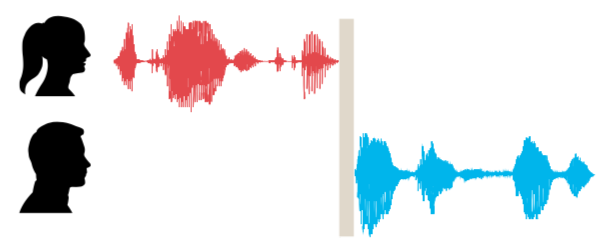
\includegraphics[width=0.5\textwidth]{../aux/img/dummy_basic_concepts.png}
	\end{columns}
}


\section{Method}%%%%
\frame{
	\frametitle{Video Material}
	\begin{figure}
		\center
		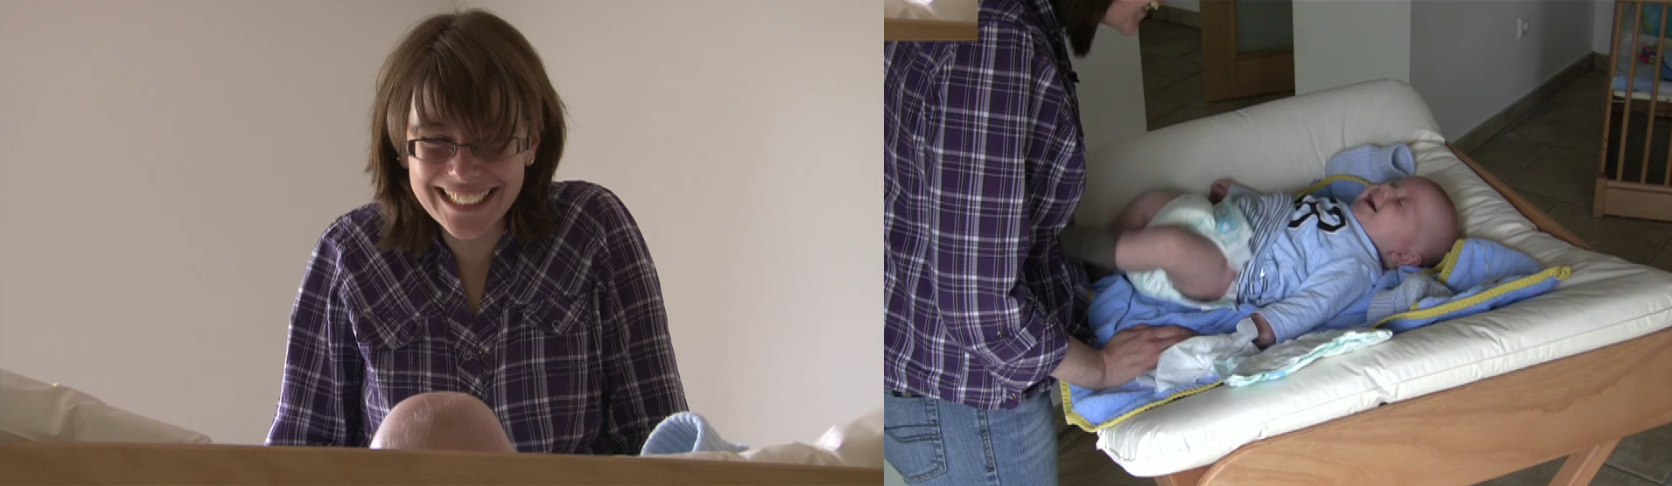
\includegraphics[width=\textwidth]{../aux/img/video_vp_08_compact.png}
		\caption{Raw Video Material}
	\end{figure}
}
\frame{
	\frametitle{Annotating the Videos}
	\begin{figure}
		\center
		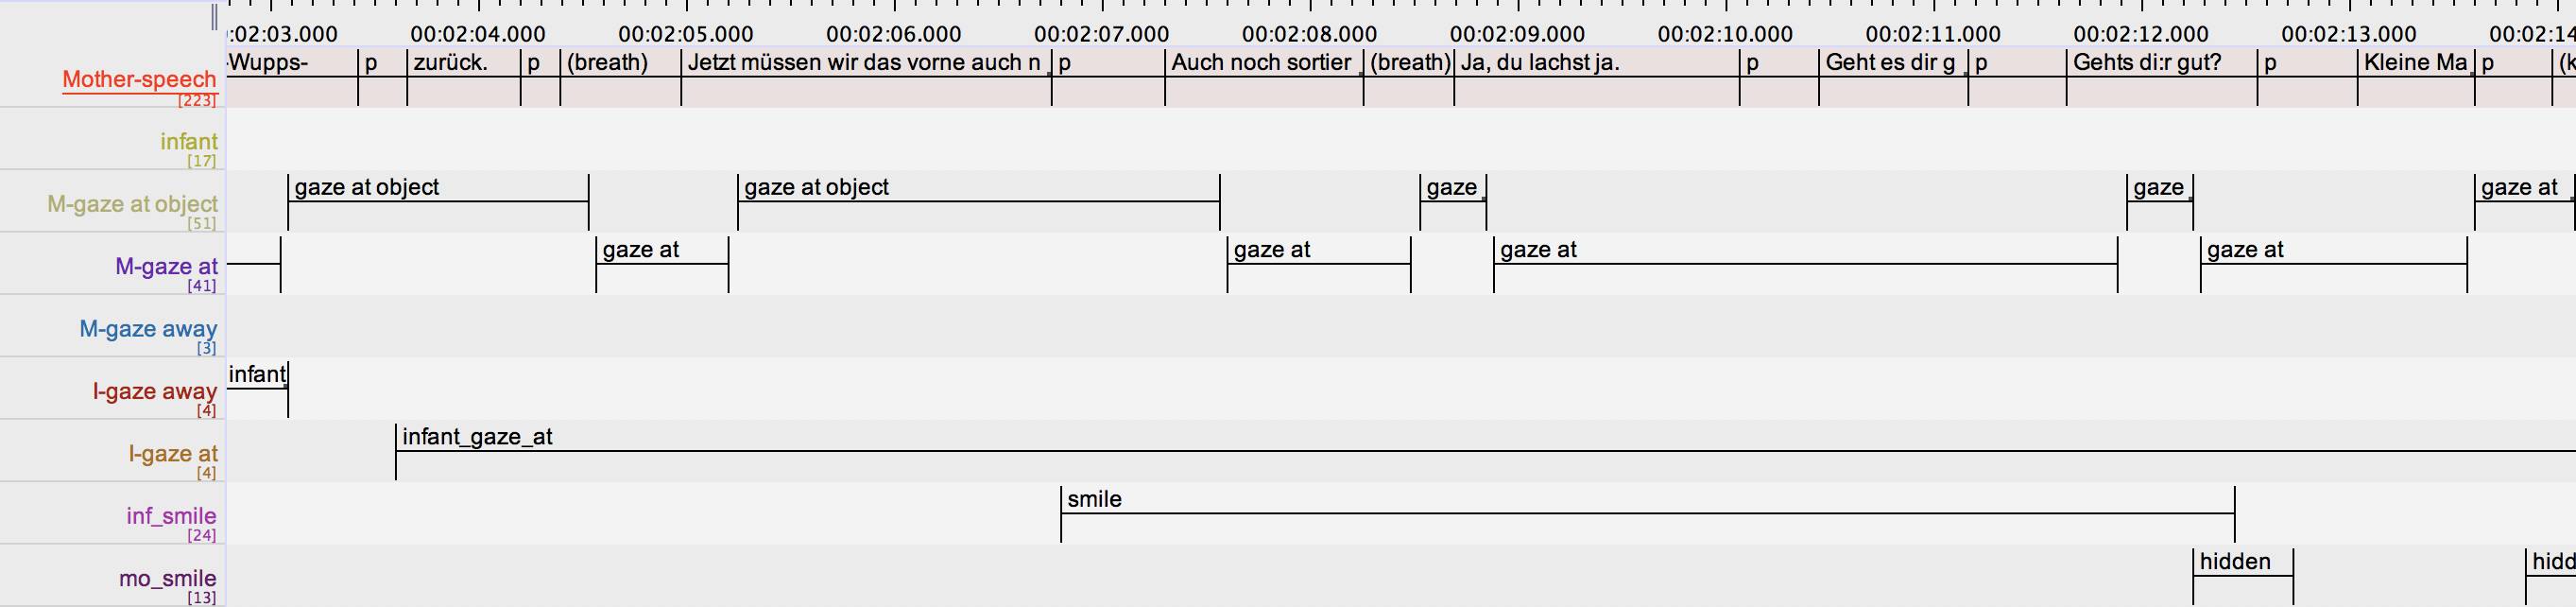
\includegraphics[width=\textwidth]{../aux/img/elan_03_cut.png}
		\caption{\textsc{elan} Screenshot}
	\end{figure}
}
\frame{
	\frametitle{What counts as a rule?}
	\begin{columns}
		\column{0.4\textwidth}
		\begin{enumerate}
			\item[]\fpmlabel{A} \rightarrow \fpmlabel{B} represents one of two cases:\textsuperscript{[1]}
			\item[]\fpmlabel{B} begins before \fpmlabel{A} ends \emph{and}
			\item interval of \fpmlabel{A} starts before interval of \fpmlabel{B} \emph{or}
			\item interval of \fpmlabel{A} and \fpmlabel{B} start at the same time
		\end{enumerate}
		\column{0.6\textwidth}
		\begin{figure}
			% !TEX root = ../../beamer/ba_beamer_master.tex
% @author Marcel Ruland (2018)
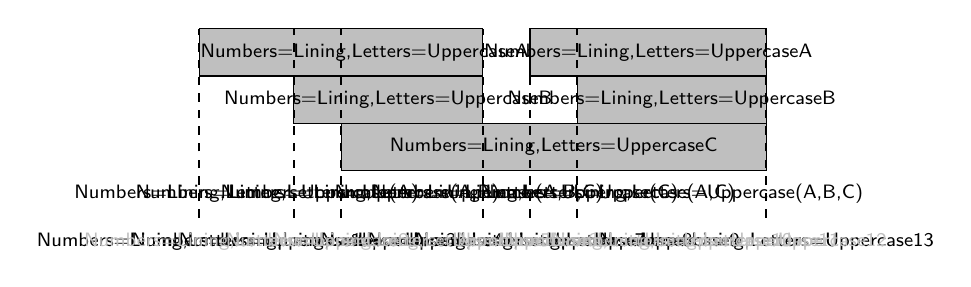
\begin{tikzpicture}[
	scale=0.6,
	every node/.append style={font=\scriptsize\sffamily\addfontfeature{Numbers=Lining,Letters=Uppercase}}]
	% boxes
	\draw [fill=lightgray] (0,4) rectangle (6,5);  % A1
	\node at (3.5,4.5) {A};
	
	\draw [fill=lightgray] (7,4) rectangle (12,5);  % A2
	\node at (9.5,4.5) {A};
	
	\draw [fill=lightgray] (2,3) rectangle (6,4);  % B1
	\node at (4,3.5) {B};
	
	\draw [fill=lightgray] (8,3) rectangle (12,4);  % B2
	\node at (10,3.5) {B};
	
	\draw [fill=lightgray] (3,2) rectangle (12,3);  % C
	\node at (7.5,2.5) {C};
	
	% item sets
	\node at (1,1.5) {(A)};
	\node at (2.5,1.5) {(A,B)};
	\node at (4.5,1.5) {(A,B,C)};
	\node at (6.5,1.5) {(C)};
	\node at (7.5,1.5) {(A,C)};
	\node at (10,1.5) {(A,B,C)};
	
	% time points
	\foreach \i in {1, 3, 4, 7, 8, 9, 13}
		\node at ({\i-1},0.5) {\i};
	\foreach \i in {2, 5, 6, 10, 11, 12}
		\node[lightgray] at ({\i-1},0.5) {\i};

	% time point lines
	\draw [dashed, thick] (0,1) -- (0,5);
	\draw [dashed, thick] (2,1) -- (2,5);
	\draw [dashed, thick] (3,1) -- (3,5);
	\draw [dashed, thick] (6,1) -- (6,5);
	\draw [dashed, thick] (7,1) -- (7,5);
	\draw [dashed, thick] (8,1) -- (8,5);
	\draw [dashed, thick] (12,1) -- (12,5);
\end{tikzpicture}
		\end{figure}
	\end{columns}
	
	\vfill
	
	{\tiny\textsuperscript{[1]}\textsc{Rohlfing}, Katharina; \textsc{Leonardi}, Giuseppe; \textsc{Hüllermeier}, Eyke; \textsc{Raczaszek-Leonardi}, Johanna; and \textsc{Nomikou}, Iris (under review): ``Multimodal turn-taking: Motivations, methodical challenges and first approaches.'' \textit{IEEE Transactions on Cognitive and Developmental Systems.}}  % decrease spacing!
}
\frame{
	\frametitle{Metrics}
	\begin{columns}
		\column{0.4\textwidth}
		\begin{itemize}
			\item confidence \\ \(conf(\mathcal{A} \rightarrow \mathcal{B}) = \frac{d(\mathcal{A}\mathcal{B})}{d(\mathcal{A})}\)
			\item absolute number of occurrences
			\item duration (\textit{sec})
		\end{itemize}
		\column{0.6\textwidth}
		\begin{figure}
			% !TEX root = ../../beamer/ba_beamer_master.tex
% @author Marcel Ruland (2018)
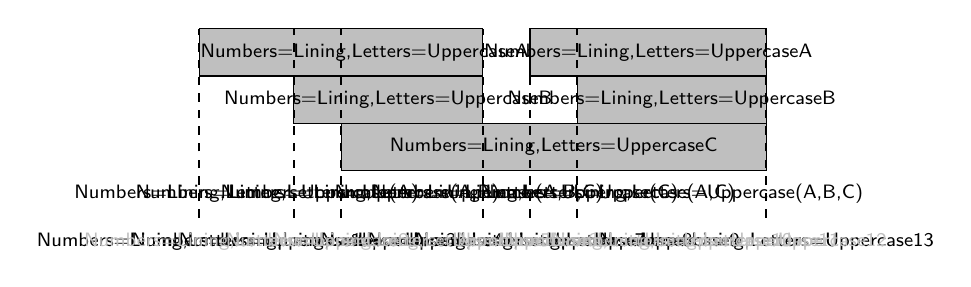
\begin{tikzpicture}[
	scale=0.6,
	every node/.append style={font=\scriptsize\sffamily\addfontfeature{Numbers=Lining,Letters=Uppercase}}]
	% boxes
	\draw [fill=lightgray] (0,4) rectangle (6,5);  % A1
	\node at (3.5,4.5) {A};
	
	\draw [fill=lightgray] (7,4) rectangle (12,5);  % A2
	\node at (9.5,4.5) {A};
	
	\draw [fill=lightgray] (2,3) rectangle (6,4);  % B1
	\node at (4,3.5) {B};
	
	\draw [fill=lightgray] (8,3) rectangle (12,4);  % B2
	\node at (10,3.5) {B};
	
	\draw [fill=lightgray] (3,2) rectangle (12,3);  % C
	\node at (7.5,2.5) {C};
	
	% item sets
	\node at (1,1.5) {(A)};
	\node at (2.5,1.5) {(A,B)};
	\node at (4.5,1.5) {(A,B,C)};
	\node at (6.5,1.5) {(C)};
	\node at (7.5,1.5) {(A,C)};
	\node at (10,1.5) {(A,B,C)};
	
	% time points
	\foreach \i in {1, 3, 4, 7, 8, 9, 13}
		\node at ({\i-1},0.5) {\i};
	\foreach \i in {2, 5, 6, 10, 11, 12}
		\node[lightgray] at ({\i-1},0.5) {\i};

	% time point lines
	\draw [dashed, thick] (0,1) -- (0,5);
	\draw [dashed, thick] (2,1) -- (2,5);
	\draw [dashed, thick] (3,1) -- (3,5);
	\draw [dashed, thick] (6,1) -- (6,5);
	\draw [dashed, thick] (7,1) -- (7,5);
	\draw [dashed, thick] (8,1) -- (8,5);
	\draw [dashed, thick] (12,1) -- (12,5);
\end{tikzpicture}
		\end{figure}
	\end{columns}
}


\section{Establishing Significance}%%%
\frame{
	\center
	\only<1>{
		{\Huge Why Significance?}
	}
	\only<2>{
		{\Huge Why Significance?}
		
		\vspace{0.2\textheight}
		
		\tikz\node[draw, rounded corners, inner sep=1em] {\LARGE qualitative \hspace{0.3\textwidth} quantitative};
	}
}
\frame{
	\frametitle{Significance -- How?}
	\begin{figure}
		% !TEX root = ../../beamer/ba_beamer_master.tex
% @author Marcel Ruland (2018)
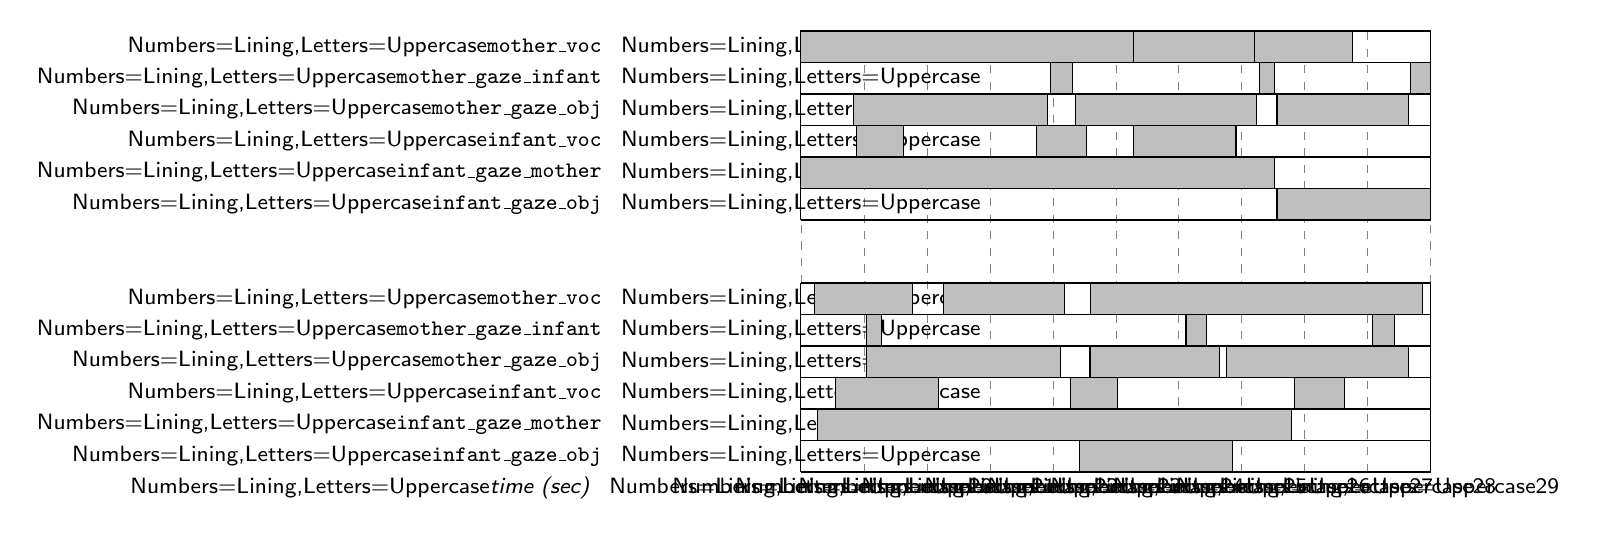
\begin{tikzpicture}[
	scale=0.8,
	node distance=0 and 0,  % y, x for fuck knows what reason
	every node/.append style={font=\footnotesize\sffamily\addfontfeature{Numbers=Lining,Letters=Uppercase}}]
%	\draw [help lines, dashed] (0,0) grid (13,7);
	
	% time line
	\node (twenty) at (3,-0.25) {20};
	\node [left=of twenty] {\textit{time (sec)}};
	\node at (4,-0.25) {21};
	\node at (5,-0.25) {22};
	\node at (6,-0.25) {23};
	\node at (7,-0.25) {24};
	\node at (8,-0.25) {25};
	\node at (9,-0.25) {26};
	\node at (10,-0.25) {27};
	\node at (11,-0.25) {28};
	\node at (12,-0.25) {29};
%	\node at (13,-0.25) {30};  % overfull hbox
	\draw [help lines, dashed] (3,3) -- (3,4);
	\draw [help lines, dashed] (4,0) -- (4,7);
	\draw [help lines, dashed] (5,0) -- (5,7);
	\draw [help lines, dashed] (6,0) -- (6,7);
	\draw [help lines, dashed] (7,0) -- (7,7);
	\draw [help lines, dashed] (8,0) -- (8,7);
	\draw [help lines, dashed] (9,0) -- (9,7);
	\draw [help lines, dashed] (10,0) -- (10,7);
	\draw [help lines, dashed] (11,0) -- (11,7);
	\draw [help lines, dashed] (12,0) -- (12,7);
	\draw [help lines, dashed] (13,3) -- (13,4);
	
	% top grid
	\draw (3,4) -- (3,7);
	\draw (13,4) -- (13,7);
	\draw (3,4) -- (13,4);
	\draw (3,4.5) -- (13,4.5);
	\draw (3,5) -- (13,5);
	\draw (3,5.5) -- (13,5.5);
	\draw (3,6) -- (13,6);
	\draw (3,6.5) -- (13,6.5);
	\draw (3,7) -- (13,7);
	
	% bottom grid
	\draw (3,0) -- (3,3);
	\draw (13,0) -- (13,3);
	\draw (3,0) -- (13,0);
	\draw (3,0.5) -- (13,0.5);
	\draw (3,1) -- (13,1);
	\draw (3,1.5) -- (13,1.5);
	\draw (3,2) -- (13,2);
	\draw (3,2.5) -- (13,2.5);
	\draw (3,3) -- (13,3);
	
	% top labels
	\node (mothervoctop) at (3,6.75) {};
	\node (mothergazeinfanttop) at (3,6.25) {};
	\node (mothergazeobjtop) at (3,5.75) {};
	\node (infantvoctop) at (3,5.25) {};
	\node (infantgazemothertop) at (3,4.75) {};
	\node (infantgazeobjtop) at (3,4.25) {};
	\node [left=of mothervoctop] {\code{mother\_voc}};
	\node [left=of mothergazeinfanttop] {\code{mother\_gaze\_infant}};
	\node [left=of mothergazeobjtop] {\code{mother\_gaze\_obj}};
	\node [left=of infantvoctop] {\code{infant\_voc}};
	\node [left=of infantgazemothertop] {\code{infant\_gaze\_mother}};
	\node [left=of infantgazeobjtop] {\code{infant\_gaze\_obj}};
	
	% bottom labels
	\node (mothervocbottom) at (3,2.75) {};
	\node (mothergazeinfantbottom) at (3,2.25) {};
	\node (mothergazeobjbottom) at (3,1.75) {};
	\node (infantvocbottom) at (3,1.25) {};
	\node (infantgazemotherbottom) at (3,0.75) {};
	\node (infantgazeobjbottom) at (3,0.25) {};
	\node [left=of mothervocbottom] {\code{mother\_voc}};
	\node [left=of mothergazeinfantbottom] {\code{mother\_gaze\_infant}};
	\node [left=of mothergazeobjbottom] {\code{mother\_gaze\_obj}};
	\node [left=of infantvocbottom] {\code{infant\_voc}};
	\node [left=of infantgazemotherbottom] {\code{infant\_gaze\_mother}};
	\node [left=of infantgazeobjbottom] {\code{infant\_gaze\_obj}};
	
	% top annotations
	\draw [fill=lightgray] (3,6.5) rectangle (8.279,7);
	\draw [fill=lightgray] (8.279,6.5) rectangle (10.206,7);
	\draw [fill=lightgray] (10.206,6.5) rectangle (11.76,7);

	\draw [fill=lightgray] (6.96,6) rectangle (7.32,6.5);
	\draw [fill=lightgray] (10.28,6) rectangle (10.52,6.5);
	\draw [fill=lightgray] (12.68,6) rectangle (13,6.5);
	
	\draw [fill=lightgray] (3.84,5.5) rectangle (6.92,6);
	\draw [fill=lightgray] (7.36,5.5) rectangle (10.24,6);
	\draw [fill=lightgray] (10.56,5.5) rectangle (12.64,6);
	
	\draw [fill=lightgray] (3.887,5) rectangle (4.624,5.5);
	\draw [fill=lightgray] (6.74,5) rectangle (7.53,5.5);
	\draw [fill=lightgray] (8.279,5) rectangle (9.909,5.5);
	
	\draw [fill=lightgray] (3,4.5) rectangle (10.52,5);

	\draw [fill=lightgray] (10.56,4) rectangle (13,4.5);

	% bottom annotations
	\draw [fill=lightgray] (7.592,2.5) rectangle (12.871,3);
	\draw [fill=lightgray] (5.264,2.5) rectangle (7.191,3);
	\draw [fill=lightgray] (3.221,2.5) rectangle (4.775,3);

	\draw [fill=lightgray] (12.069,2) rectangle (12.429,2.5);
	\draw [fill=lightgray] (4.039,2) rectangle (4.279,2.5);
	\draw [fill=lightgray] (9.115,2) rectangle (9.435,2.5);
	
	\draw [fill=lightgray] (4.04,1.5) rectangle (7.12,2);
	\draw [fill=lightgray] (9.76,1.5) rectangle (12.64,2);
	\draw [fill=lightgray] (7.59,1.5) rectangle (9.64,2);
	
	\draw [fill=lightgray] (7.287,1) rectangle (8.024,1.5);
	\draw [fill=lightgray] (10.84,1) rectangle (11.63,1.5);
	\draw [fill=lightgray] (3.55,1) rectangle (5.18,1.5);
	
	\draw [fill=lightgray] (3.27,0.5) rectangle (10.79,1);

	\draw [fill=lightgray] (7.42,0) rectangle (9.86,0.5);
\end{tikzpicture}
	\end{figure}
}

\section{Results}
\frame{
	\frametitle{Results}
}
%\frame{
%	\frametitle{Bibliography}
%	\bibliography{../bib/ba_bib}
%}
\end{document}

%\frame{
%	\frametitle{Dummy}
%	\begin{columns}
%		\columns{0.5\textwidth}
%			left
%		\columns{0.5\textwidth}
%			right
%	\end{columns}
%}
